Набор данных MOTChallenge \cite{dendorfer2021motchallenge} является одним из наиболее популярных в области для сравнения между собой различных алгоритмов отслеживания нескольких объектов на видеоизображениях одновременно. 
Со дня своего появления он быстро обрел статус стандарта индустрии. 

Бенчмарк MOT17 был выпущен в 2017 году и является идейным наследником более ранних версий -- MOT15 и MOT16. В ходе этого развития авторами был исправлен ряд проблем старых версий:
\begin{itemize}
    \item[--] с развитием технологии отслеживания объектов на изображении MOT15 стал слишком простым для современных методов. MOT16 начал включать в себя ряд новых видео, где траектории объектов чаще пересекаются друг с другом, условия освещения более разнообразны, а средняя плотность объектов на изображении увеличилась в три раза;
    \item[--] MOT17 решает другую важную проблему -- уточняет разметку набора данных, так как в предыдущей версии нередко встречались ошибки. 
\end{itemize}

В итоге MOT17 включается в себя 14 различных видео общей протяженностью порядка 4 минут. Все они представляют из себя различные записи с уличных камер, на которых пешеходы перемещаются по тротуарам, площадям, торговым центрах. 
В наборе данных представлены различные ракурсы: как видео с подвижной камерой снятые человеком, находящимся в толпе, так и сделанные с возвышенности статично, например, камерой наблюдения.

На рисунках \ref{fig:mot_1}-\ref{fig:mot_3} приведены примеры изображений из бенчмарка.

\begin{figure}[ht]
    \centering
    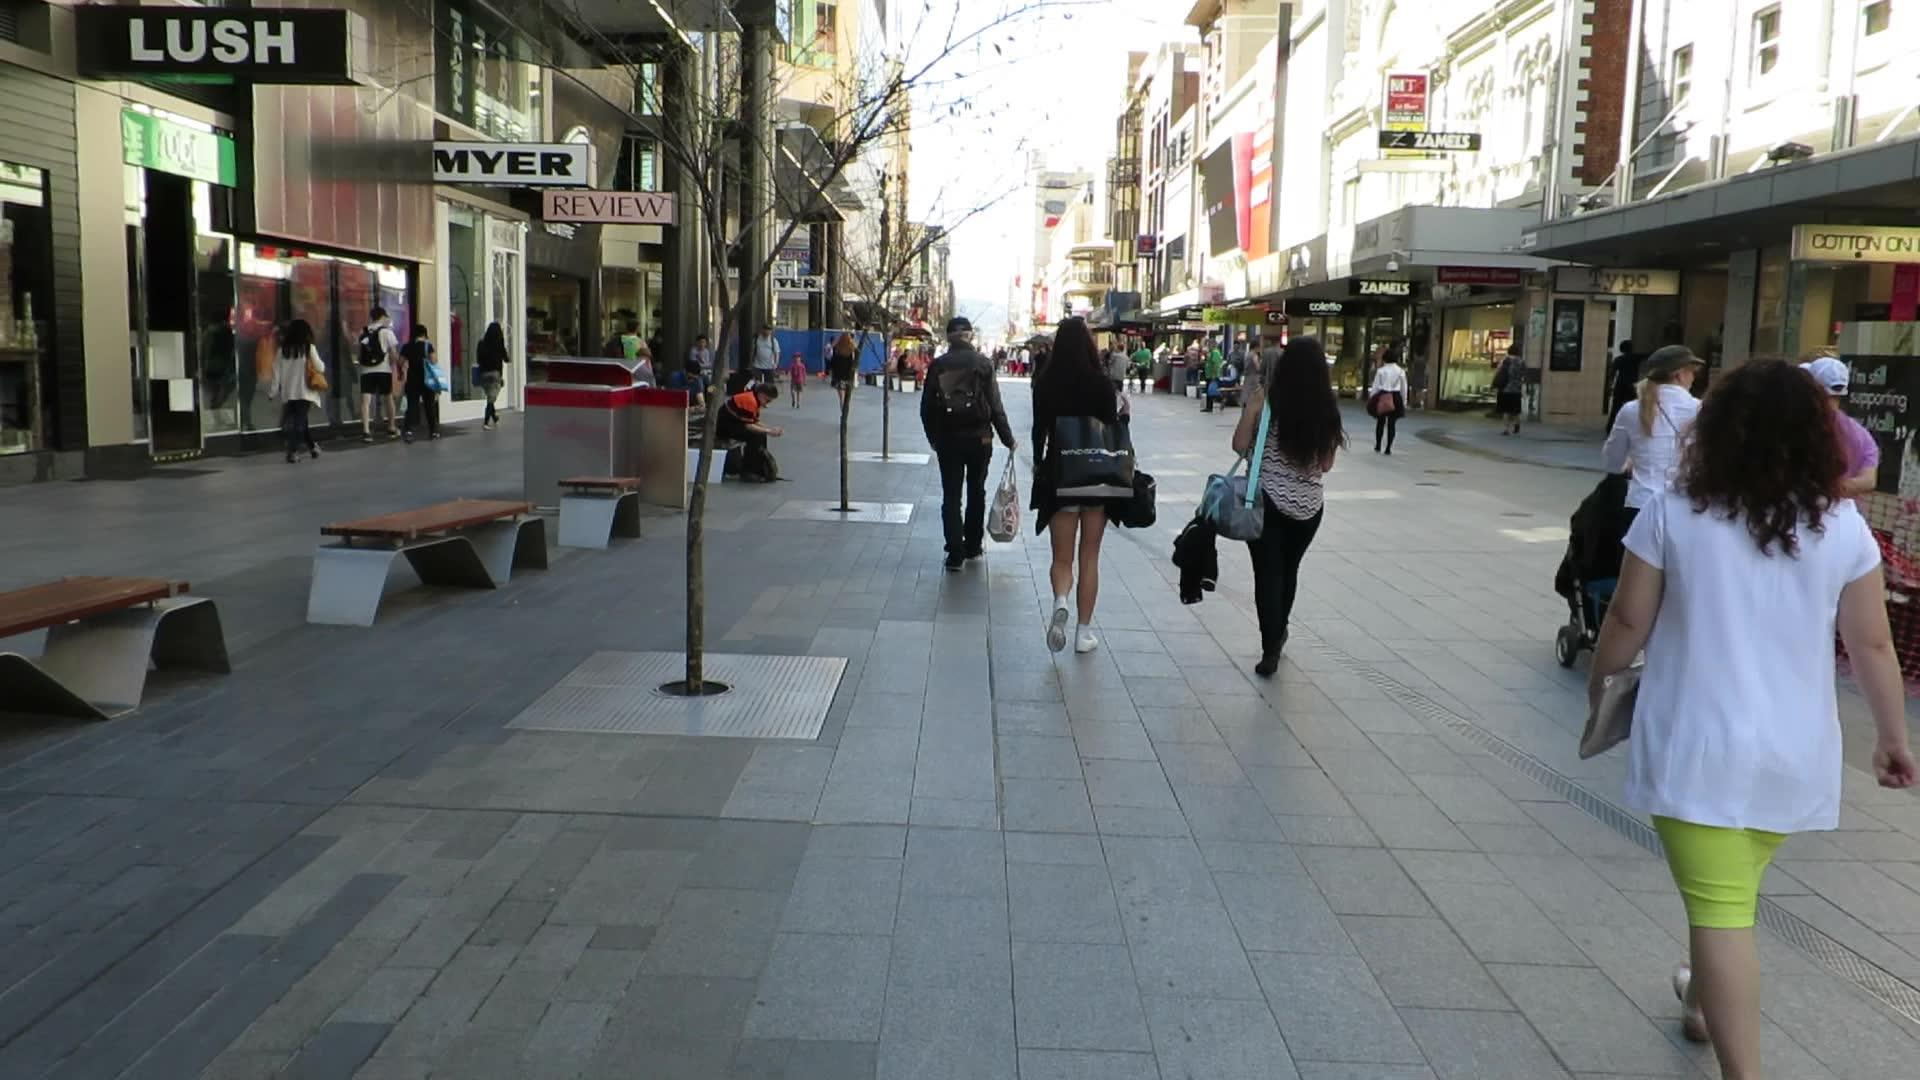
\includegraphics[width=0.7\textwidth]{review/MOT17_1}
    \caption{Пример изображения из набора данных MOT17 (приводится по \cite{dendorfer2021motchallenge}, страница 850, рисунок 3).}
    \label{fig:mot_1}
\end{figure}

\begin{figure}[ht]
    \centering
    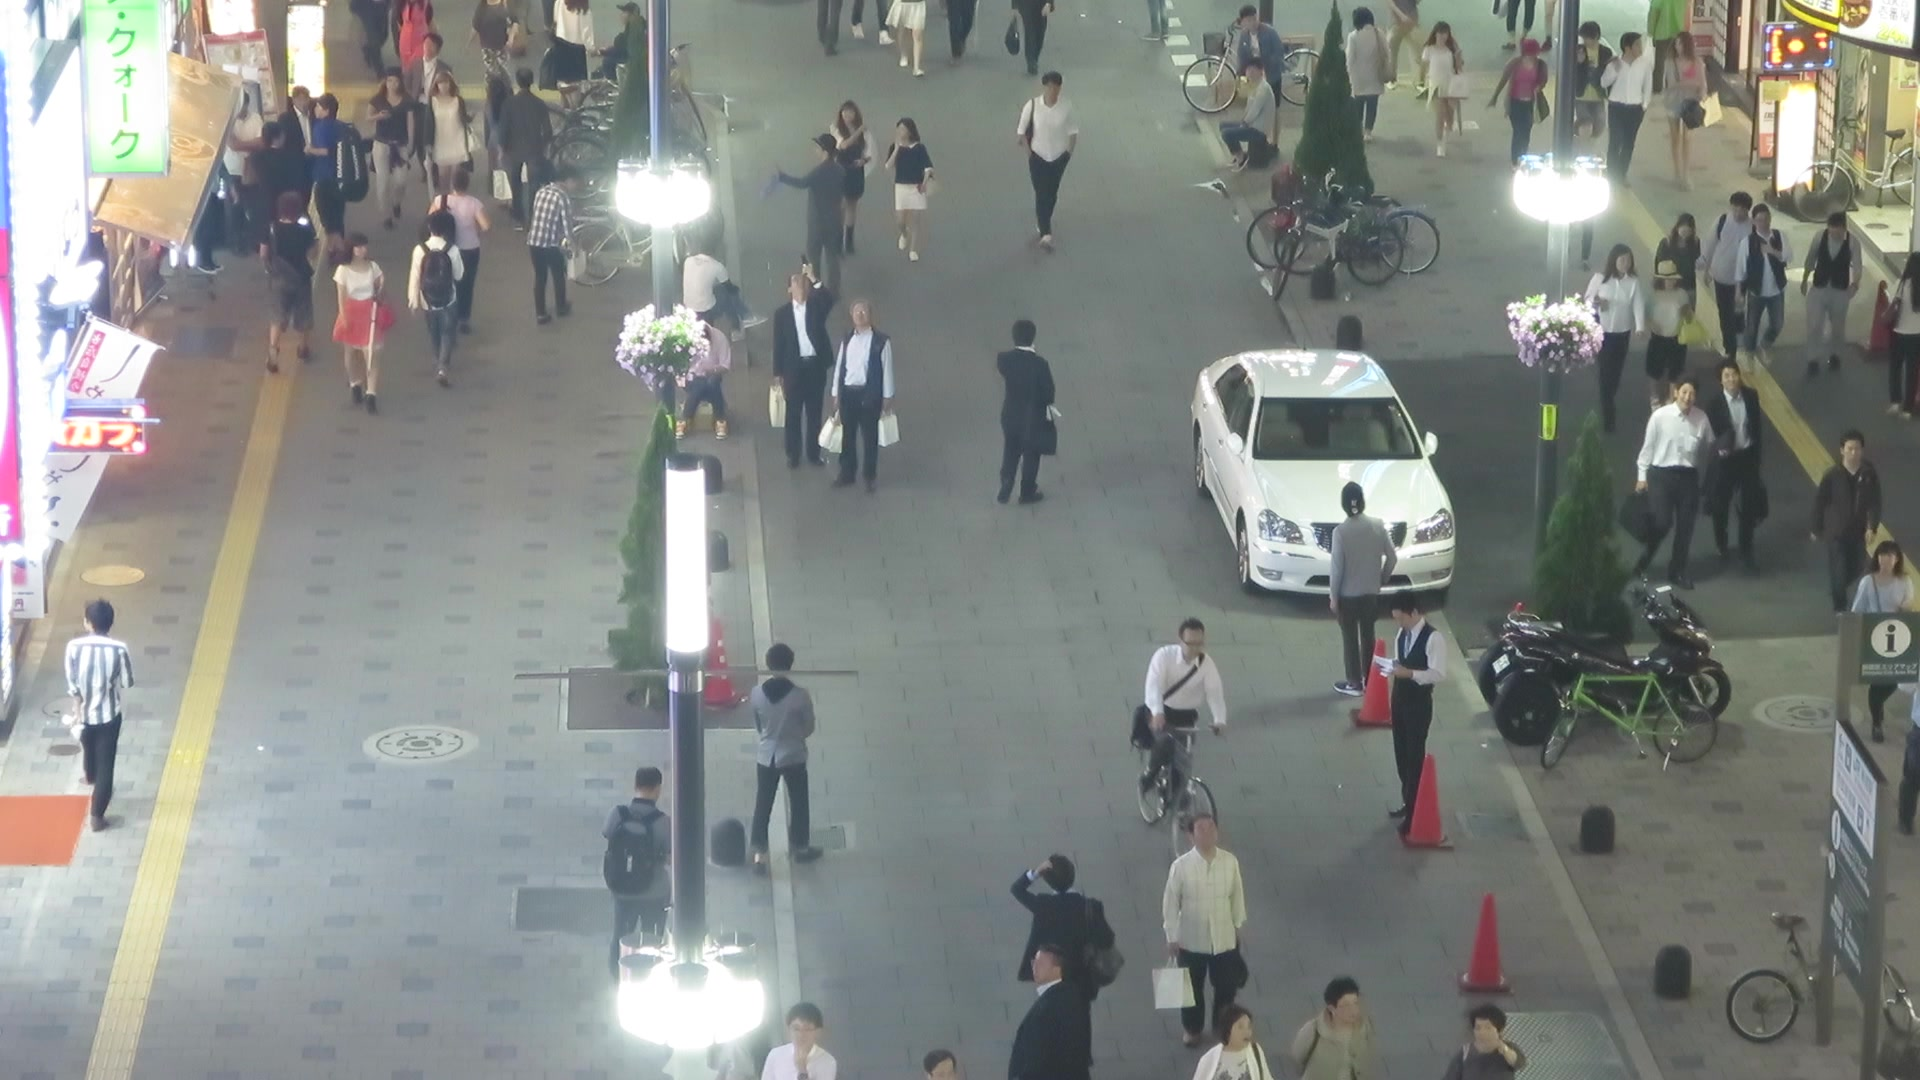
\includegraphics[width=0.7\textwidth]{review/MOT17_2}
    \caption{Пример изображения из набора данных MOT17 (приводится по \cite{dendorfer2021motchallenge}, страница 850, рисунок 3).}
    \label{fig:mot_2}
\end{figure}

\begin{figure}[ht]
    \centering
    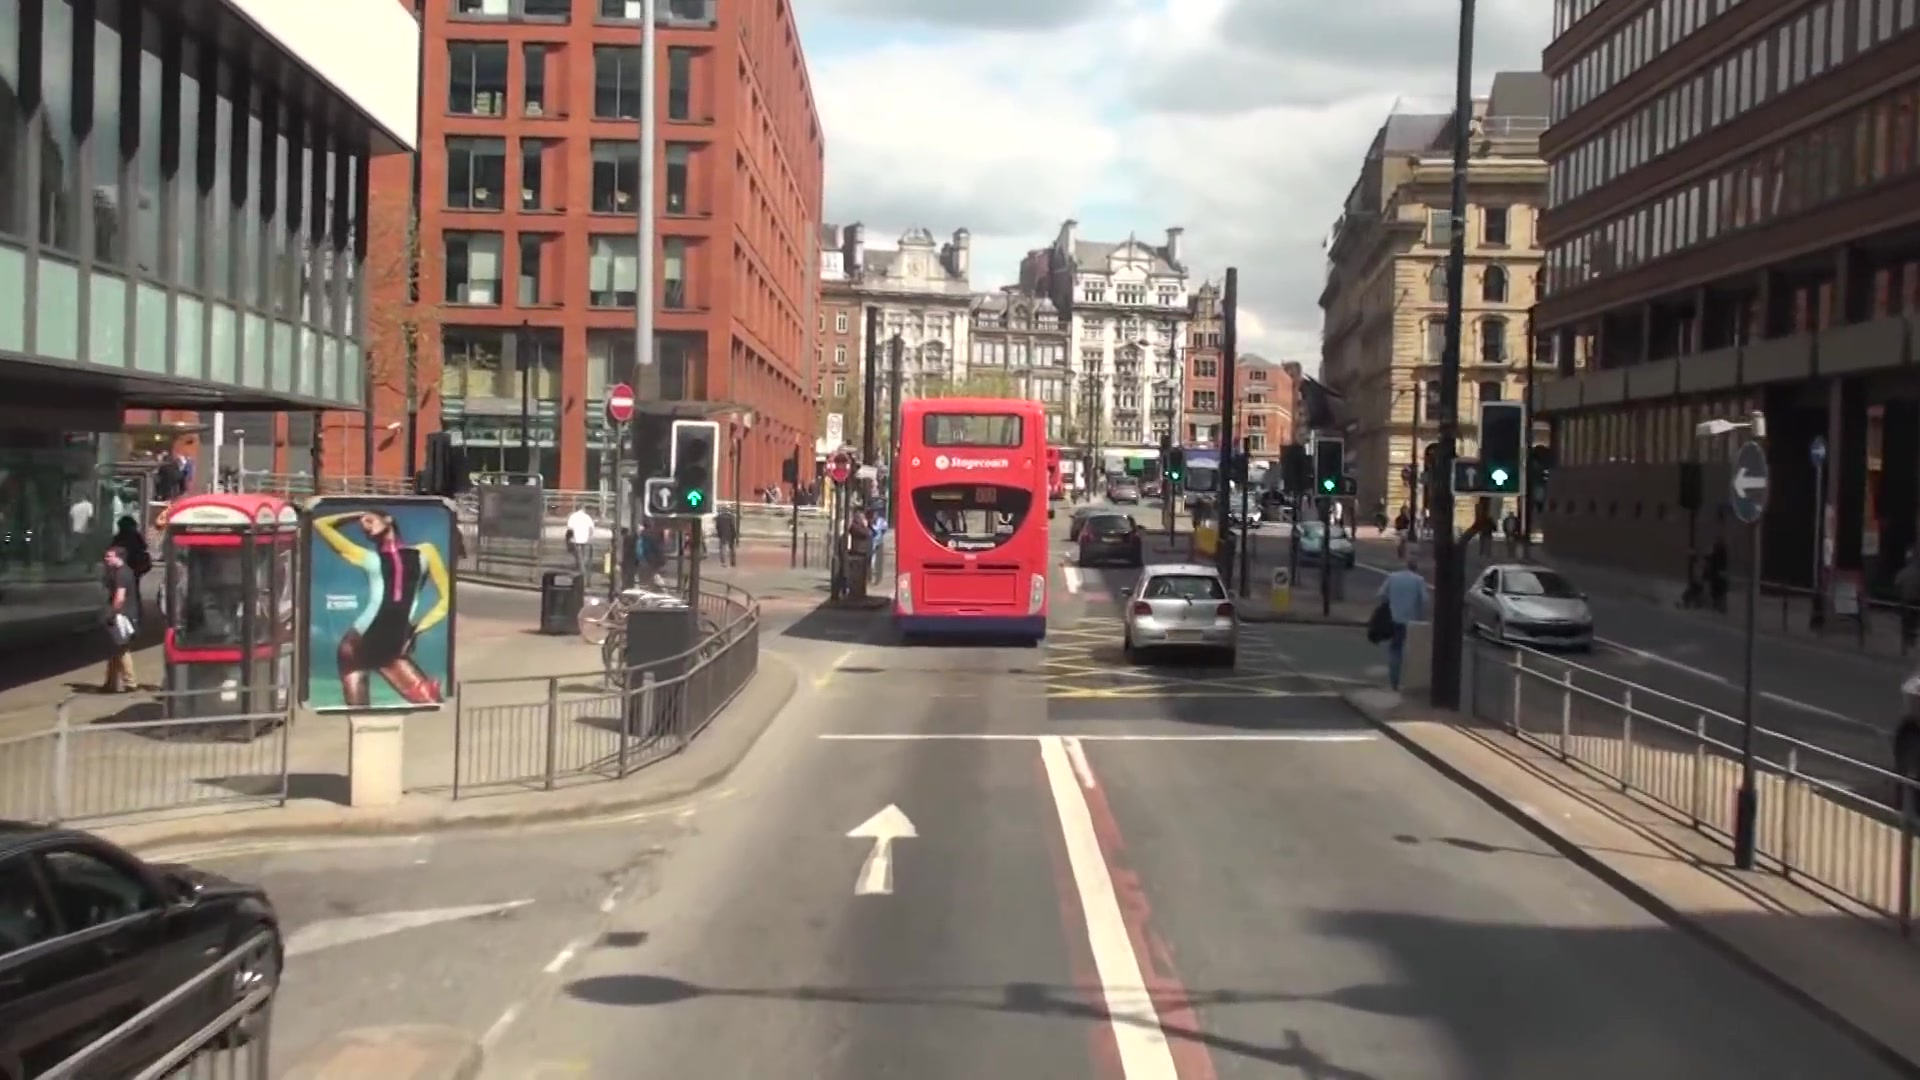
\includegraphics[width=0.7\textwidth]{review/MOT17_3}
    \caption{Пример изображения c из набора данных MOT17(приводится по \cite{dendorfer2021motchallenge}, страница 850, рисунок 3).}
    \label{fig:mot_3}
\end{figure}

\FloatBarrier